% anstelle von article auch KOMA-Skript-Variante scrartcl
\documentclass[11pt]{article}
%anstelle von german auch ngerman
\usepackage{amsfonts,latexsym,eurofont,ngerman}
\usepackage{graphicx,color}

\usepackage[T1]{fontenc}
\usepackage[utf8]{inputenc}
\usepackage[ngerman]{babel}
\usepackage{fancyhdr} 

%titelblatt
\thispagestyle{empty}

\setlength{\textheight} {250mm} 
\setlength{\textwidth} {150mm}

%Kopfzeile
\setlength{\topmargin} {-25mm}

%Fußzeile
%\setlength{\footheight} {10mm}
\setlength{\footskip} {10mm}


%Seiten link
\setlength{\oddsidemargin} {10mm} 

%Seite rechts und Rand
\setlength{\marginparwidth} {0mm} 
\setlength{\marginparsep} {0mm} 

%Absätze nicht einrücken, möglicherweise nicht zu empfehlen, falls viele Abbildungen vorhanden;
%Betreuer fragen
\parindent10mm

% Kopf- und Fußzeilen anpassen
\fancyhf{}  % Kopf- und Fußzeile leeren 
\fancyfoot[EL]{\thepage} 
\fancyfoot[OR]{\thepage} 
\pagestyle{fancy} 


%Inhaltsverzeichnis
\usepackage[numindex,nottoc,section]{tocbibind} %Einbinden von Index-
                                %und Literaturverzeichnis (nummeriert) in das
                                %Inhaltsverzeichnis. Inhaltsverzeichnis wird 
                                %nicht eingebunden.

\usepackage{eso-pic,graphicx}
\usepackage{hyperref}
\hypersetup{pageanchor,linkcolor=black, colorlinks=true}

\makeatletter

\newcommand\BackgroundPicture[3]{%
  \setlength{\unitlength}{1pt}%
  \put(0,\strip@pt\paperheight){%
    \parbox[t][\paperheight]{\paperwidth}{%
      \vfill
      \centering
\includegraphics[width=21.4cm,angle=45]{_Res/draft}
      \vfill
    }
  }
} 

\makeatother
\AddToShipoutPicture{\BackgroundPicture}
\usepackage{eso-pic,graphicx}
\usepackage{hyperref}
\hypersetup{backref,pageanchor,hyperindex=true,linkcolor=darkblue, colorlinks=true}

\makeatletter

\newcommand\BackgroundPicture[3]{%
  \setlength{\unitlength}{1pt}%
  \put(0,\strip@pt\paperheight){%
    \parbox[t][\paperheight]{\paperwidth}{%
      \vfill
      \centering
\includegraphics[width=21.4cm,angle=45]{_Res/draft}
      \vfill
    }
  }
} 

\makeatother
\AddToShipoutPicture{\BackgroundPicture}

\begin{document}


\begin{titlepage}
\author{}
%Bilder einfügen
\begin{figure}[hp]
	\centering
	
\includegraphics[height = 13mm]{./_Res/RAC_Logo.jpg}
\end{figure}
\begin{center}
\huge
\textsc{Übersetzen von Schrittmotorprotokollen\\ mittels Mikrocontroller}\\

\vspace{2cm}

\LARGE
%\textsc{\bf Bachelorarbeit\\[0.5\baselineskip]
\textsc{\bf Praxisprojektbericht\\[0.5\baselineskip]
\Large \normalfont {im Studiengang Mess- und Sensortechnik\\[0.5\baselineskip]
Fachhochschule Koblenz, RheinAhrCampus Remagen}}

\large
\vspace{2cm}
\textnormal{vorgelegt von\\[0.5\baselineskip]\textbf{Johannes Dielmann}\\[0.5\baselineskip] geb.\ am 10.01.1984 in {\em Kirchen} }\\ 
\vspace{1cm}


\end{center}

\normalsize
\begin{flushleft}	

\vspace{15mm}
\begin{tabbing}
Externer Betreuer:\quad\=\kill
Betreuer: \> Prof.\ Dr.\ Carstens-Behrens\\[1\baselineskip]

\end{tabbing}
\end{flushleft}

%\vspace{0mm} 

\vspace{4cm}

\begin{center}
\textnormal{Remagen, \today}
\end{center}


\end{titlepage}

% Erstellung des Inhaltsverzeichnisses
\tableofcontents 	\newpage
\listoffigures 		\newpage
\listoftables		\newpage
\newpage

\section{Einleitung}
\subsection{Überblick}
Gegeben war das 3D-Lasererfassungssystem VI-900 der Firma Minolta, im Folgenden kurz VI-900 genannt, und ein Drehtisch. Der Drehtisch dient zur Aufnahme des zu erfassenden Objektes aus allen Richtungen. Des weiteren lässt sich das 3D-Modell später in der Software wesentlich einfacher zusammenführen wenn der Drehtisch benutzt wird.\\
Dem VI-900 lag die Software RapidForm2004 bei. Mit dieser Software lassen sich 3D-Modelle einfach bearbeiten und einzelne Modelle zu einem gesamten zusammenführen. Diese Software spricht sowohl das VI-900 an als auch den Drehtisch. \\
In RapidForm2004 sind jedoch nur einige wenige Schrittmotoren und deren Protokolle hinterlegt.
\subsection{Aufgabenstellung}
Mit dem Aufbau aus RapidForm2004, Lasererfassungssystem und Drehtisch sollen auf einfachem Wege 3D-Modelle eines Objektes erzeugt werden und diese dann zur Vermessung oder zur weiteren Verwendung in CAD-Software herangezogen werden.\\
Um ein vollständiges und brauchbares 3D-Objekt zu erhalten kann die Software einen Drehtisch ansteuern.\\
Da das Protokoll des Drehtisches nicht kompatibel zu denen in der Software war musste das Protokoll also übersetzt werden.\\
\subsection{Problemlösung}
Da die Kommunikation mittels ASCII-Zeichen über die RS-232 Schnittstelle des Computers erfolgt, lässt sich die Information leicht mit einem Mikrocontroller abfangen, auswerten und richtig kodiert an die Ansteuerung des Drehtisches weitersenden.
Benötigt wird also ein Mikrocontroller mit 2 RS-232 Schnittstellen. Um später den Ablauf anzeigen zu können und den Drehtisch auch manuell bedienen zu können wurde noch ein LC-Display und mehrere Bedientaster eingeplant.\\
Da die Ansteuerung des Schrittmotors als Einschub für ein 19"-Rack realisiert ist wählte ich für den Mikrocontroller auch die realisierung als 19"-Einschubplatine.
\newpage

\section{Projektaufbau}
\subsection{Übersicht}
\begin{figure}[hp]
	\centering
	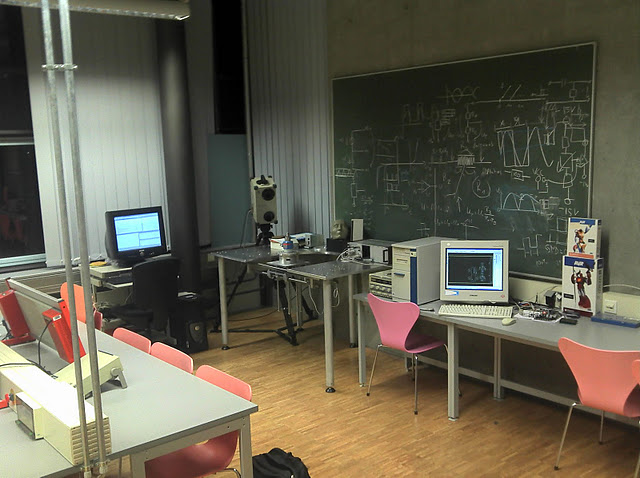
\includegraphics[width=16cm]{./_Res/Uebersicht.jpg}
	\caption{Übersicht}
\end{figure}
\subsection{Die einzelnen Komponenten}
\subsubsection{Lasererfassungssystem VI-900}
\subsubsection{Ansteuerung für Drehtisch}
\subsubsection{Drehtisch}
\subsubsection{Arbeitsplatz Rechner}
\newpage

\addcontentsline{toc}{section}{A Anhang 1}
\section*{A Anhang 1}
\newpage

\begin{thebibliography}{99}
%Zeitschriftenartikel
\bibitem{maquarbra} Mack, T., Quarg, G., Braun, C.\ (2006). {\em The mean square error of prediction in the chain ladder reserving method. A comment.} ASTIN Bulletin 36, 543-553. 
%Buch
\bibitem{mik} Mikosch, T.\ (1994). {\em Non-life insurance mathematics.} Springer, Heidelberg.
%Internetquelle
\bibitem{wiki1} Wikipedia. {\em Chi--Quadrat--Test}, http://de.wikipedia.org/wiki/Chi-Quadrat-Test, Stand: 30.09.2011.
\end{thebibliography}
\newpage

\section*{Erklärung}

\vspace{2cm}

Hiermit versichere ich, dass ich den vorliegenden Bericht selbständig und nur unter Verwendung der angegebenen Quellen und Hilfsmittel verfasst habe.

\vspace{2cm}

Remagen, den \today \hfill {Johannes Dielmann} 
\begin{figure}[hp]
	\hfill
	
\includegraphics[height = 13mm]{../../../../Unterschrift.png}
\end{figure}


\end{document}
